\section{Datenbank (D.R.)}
\label{sec-db}
In diesem Projekt wird das DBMS von PostgreSQL \cite{postgresql} verwendet. Dieses begründet sich einerseits durch die Kompatibilität mit EF Core \cite{ajcvickers}, ASP.NET \Cite{wadepickett} und FastAPI \cite{fastapi} andererseits
durch die äußeren Faktoren Kosten und Geschwindigkeit. ~\\
Das System läuft zusammen mit dem Backend und dem Frontend auf einem Server in einer Dockerumgebung als Container, damit eine dauerhafte Verfügbarkeit gewährleistet werden kann.
Genaueres dazu befindet sich in Kapitel \ref{sec-docker}.

\subsection{Modellierung}
\label{sec-db-modell}
Der Aufbau der Datenbank richtet sich nach den Prinzipien der Normalisierung. Anhand der semi-struktierten JSON \cite{json}  (siehe Kapitel \ref{sec-struc-json}) wurden alle Entitäten, Beziehungen und
Attribute ermittelt, so dass eine strukturierte Architektur entstanden ist. Diese wurde größtenteils bis zur dritten Normalform gestaltet. Eine Ausnahme bildet die Tabelle \textit{TBL\_STATION}.
Hier werden aus Gründen der Wartbarkeit und Perfomance zum Beispiel die Attribute \textit{LONGITUDE} und \textit{LATITUDE} in der Tabelle gelassen. Jede Tabelle besitzt aber mindestens einen Primärschlüssel und die Domänen der Attribute sind atomar. 
Zusätzlich wurden an jede Relation die Attribute \textit{UPDATE\_NAME}, \textit{UPDATE\_TS}, \textit{INSERT\_NAME} und \textit{INSERT\_TS} angehangen und die Tabelle \textit{TBL\_IMPORT} hinzugefügt. Diese werden für die Fehlerbehandlung in der Pipeline benötigt (siehe Kapitel \ref{sec-metadata-import}).
Die folgende Übersicht stellt die Beziehungen, Kardinalitäten und Attribute als ER-Diagramm dar.
\begin{figure}[H]
    \centering
    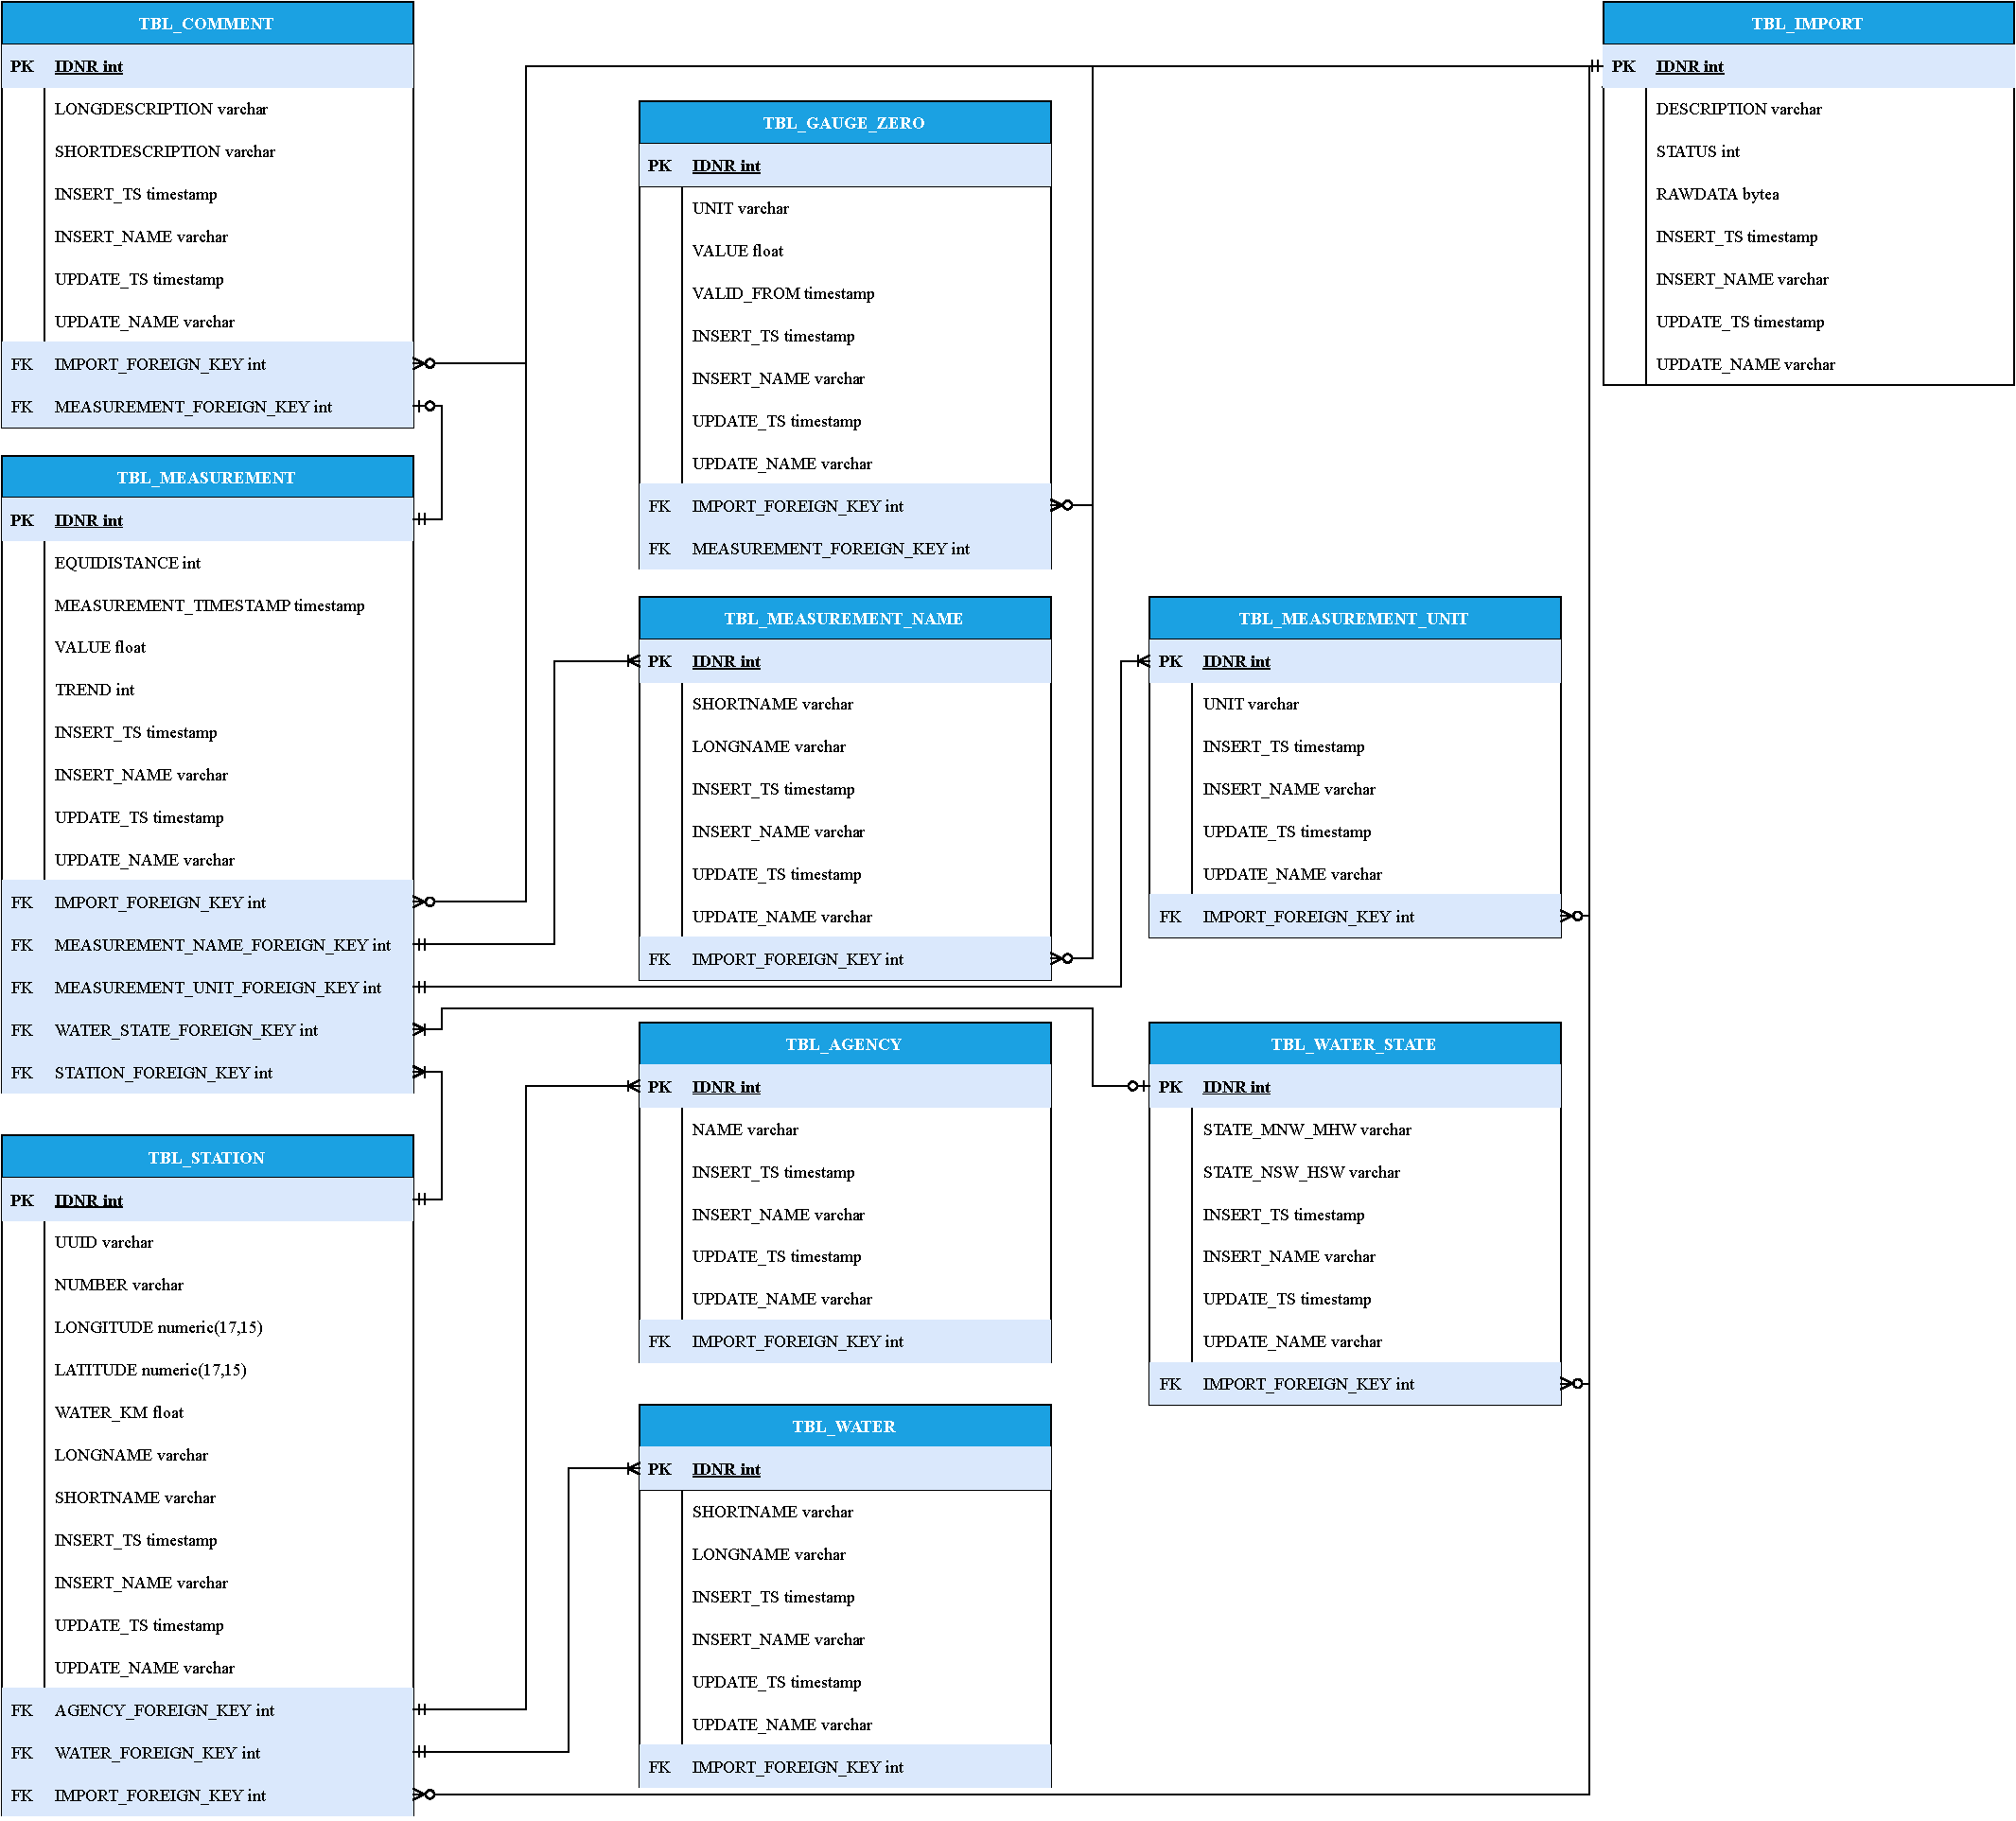
\includegraphics[width=\linewidth]{figures/ERModel.pdf}
    \label{fig:er-model-1}
    \caption{ER-Diagramm}
\end{figure}
\noindent Das eigentliche Erzeugen der Tabellen, falls diese nicht vorhanden sind, erfolgt beim Start des Postgres-Containers (vergleiche Kapitel \ref{sec-docker}). Dort wird automatisch sichergestellt, dass die Datenbank entsprechend dem Schema erstellt und 
konfiguriert ist. Dazu werden verschiedene SQL-Statements ausgeführt.
~\\
\begin{lstlisting}[language={SQL}, caption={Beispiel SQL-Statement zum Erstellen von TBL\_STATION}, captionpos=b, label={sql-tbl}]
   CREATE TABLE public."TBL_STATION" (
	"IDNR" int4 NOT NULL GENERATED BY DEFAULT AS IDENTITY,
	"UUID" varchar(255) NOT NULL,
	"LONGITUDE" numeric(17, 15) NOT NULL,
	"LONGNAME" varchar(255) NOT NULL,
	"NUMBER" varchar(255) NOT NULL,
	"LATITUDE" numeric(17, 15) NOT NULL,
	"SHORTNAME" varchar(255) NOT NULL,
	"WATER_KM" float8 NOT NULL,
	"AGENCY_FOREIGN_KEY" int4 NOT NULL,
	"WATER_FOREIGN_KEY" int4 NOT NULL,
	"IMPORT_FOREIGN_KEY" int4 NOT NULL,
	"INSERT_TS" timestamp NOT NULL,
	"INSERT_NAME" varchar(255) NOT NULL,
	"UPDATE_TS" timestamp NOT NULL,
	"UPDATE_NAME" varchar(255) NOT NULL,
	CONSTRAINT "PK_TBL_STATION" PRIMARY KEY ("IDNR")
    );
\end{lstlisting}
\subsection{Trigger und Funktionen}
Für jede Tabelle wurde ein Trigger erstellt, der nach einem Update, die in Kapitel \ref{sec-metadata-import} beschriebenen Spalten \textit{UPDATE\_NAME} und \textit{UPDATE\_TS}, automatisch füllt. 
Damit soll sichergestellt werden, dass manuelle Änderungen durch Benutzer auf Seiten des Datenbanksystems erfasst werden. Dadurch lassen sich die Ursachen für
Anomalien innerhalb der Daten eingrenzen. Außerdem wird für eine höhere Transparenz gesorgt. Um dieses Verhalten mit PostgreSQL
zu realisieren muss zusätzlich eine Funktion geschrieben werden, die das Update der Spalten durchführt. Im Gegensatz zu den Triggern reicht eine allgemeine Funktion, weil
die Änderungen global in der Variable \textit{NEW} abrufbar sind.
~\\
\begin{lstlisting}[language={SQL}, caption={Funktion für die Aktualisierung der Metadaten}, captionpos=b, label={list-function}]
CREATE FUNCTION func_update_metadata() RETURNS TRIGGER AS $trg_update_metadata$
    BEGIN
        -- Remember who changed the row
        NEW."UPDATE_TS" := current_timestamp;
        NEW."UPDATE_NAME" := current_user;
        RETURN NEW;
    END;
$trg_update_metadata$ LANGUAGE plpgsql;
\end{lstlisting}~\\
Das Erstellen der Trigger wurde anschließend für alle Tabellen durchgeführt und ist hier für die Tabelle \textit{TBL\_STATION} beispielhaft aufgeführt.
~\\
\begin{lstlisting}[language={SQL}, caption={Trigger für die Tabelle TBL\_STATION}, captionpos=b, label={list-trigger}]
    CREATE TRIGGER trg_update_metadata BEFORE UPDATE ON "TBL_STATION"
        FOR EACH ROW EXECUTE FUNCTION func_update_metadata();
\end{lstlisting}
\subsection{Konfiguration der Benutzer} 
Die Gestaltung des Rollenschemas richtet sich nach dem Minimalprinzip. Damit erhält jede Rolle nur die Berechtigungen, die sie benötigt. Insgesamt wurden folgende drei Benutzer angelegt:
\begin{itemize}
    \item \textit{postgres:} Dieser Benutzer wird beim Erstellen des DBMS von Postgres benötigt und fungiert als Admin. Damit hat er alle Rechte.
    \item \textit{update\_service:} Dieser Benutzer wurde für die Pipeline (siehe Kapitel \ref{sec-pipeline}) angelegt und hat die Berechtigungen:
    \begin{enumerate}[label=(\alph*)]
        \item SELECT
        \item UPDATE
        \item DELETE
        \item INSERT
        \item CREATE
        \item DROP
        \item ALTER
    \end{enumerate}
    \item \textit{api\_service:} Dieser Benutzer wurde für die API-Schnittstelle erstellt und hat folgende Berechtigungen:
    \begin{enumerate}[label=(\alph*)]
        \item SELECT
    \end{enumerate}
\end{itemize}
Wie in der Einleitung dieses Kapitels bereits beschrieben, läuft das Datenbanksystem in einer Dockerumgebung. Damit diese Benutzer reproduzierbar sind und automatisch beim
Start eines Containers angelegt werden, wurde ein Skript geschrieben. Dieses wird beim Start des Containers automatisch aufgerufen.
~\\
\begin{lstlisting}[language={bash}, caption={Bash zum Erstellen der SQL-Nutzer}, captionpos=b, label={list-trigger}]
#!/bin/bash
set -e

psql -v ON_ERROR_STOP=1 --username "$POSTGRES_USER" --dbname "$POSTGRES_DB" <<-EOSQL
	 CREATE USER update_service WITH PASSWORD '****';
	 GRANT ALL PRIVILEGES ON DATABASE "DB_WATER" TO update_service;
    CREATE USER api_service WITH PASSWORD '****';
    GRANT CONNECT ON DATABASE "DB_WATER" TO api_service;
    GRANT SELECT ON ALL TABLES IN SCHEMA public TO api_service;
EOSQL
\end{lstlisting}
\subsection{Datensicherung}
Die Vermeidung von Datenverlust spielt eine wichtige Rolle im Umgang mit Datenbanken. Deswegen wurde in diesem
Projekt ein Cronjob angelegt, welcher täglich ein Backup von der Datenbank macht und dieses speichert. Dadurch kann
der letzte Stand wiederhergestellt werden. Die Verwaltung der Hardware findet auf Seiten der Betreiber des Servers statt.
Die Beschreibung der Implementierung befindet sich im Kapitel \ref{sec-docker-db}.